\documentclass[10pt,a4paper]{article}
\usepackage[latin1]{inputenc}
\usepackage{amsmath}
\usepackage{amsfonts}
\usepackage{amssymb}
\usepackage{float}
\usepackage{listings}
\usepackage{graphicx}
\usepackage[usenames,dvipsnames]{color}

\begin{document}
\definecolor{light-gray}{gray}{0.90}
\lstset{language=Python,breaklines=true,backgroundcolor=\color{white},frame=single}

\author{Jeroen Hofman\\
		10194754\\
		}
\title{Computer exercises week 41, 2011\\
		}
\date{}
\maketitle

\subsection*{Exercise 7.1}
Code:
\begin{lstlisting}
def eval(n,x,t,deriv=False,inte=False,a=0,b=0):
    if deriv==False and inte==False:
        value  = x[-1]
        for j in range(2,n+2):
            value *= t
            value += x[-j]
        return value
    if deriv == True and inte==False:
        y = [0]*(len(x)-1)
        n = n-1
        for i in range(0,len(x)-1):
            y[i] = x[i+1]*(i+1)
        value = y[-1]
        for j in range(2,n+2):
            value *= t
            value += y[-j]
        return value
    if inte==True and a!=b and deriv == False:
        y = [0]*(len(x)+1)
        n = n + 1
        for i in range(1,len(x)+1):
            y[i] = float(x[i-1])/float(i)
        value1,value2 = y[-1],y[-1]
        for j in range(2,n+2):
            value1 *= a
            value2 *= b
            value1 += y[-j]
            value2 += y[-j]
        return value2-value1
    else: 
        return 'wrong input, possibly forgot integral boundaries or trying to integrate/differentiate at the same time!'

n = random.randint(0,10)
x = np.random.randint(0,10,n+1)
t = random.randint(0,10)
value = eval(n,x,t,False,True,1,2)
print value
\end{lstlisting}

\noindent In the above code we have defined a function eval, which either evaluates the function in a given point $t$, or evaluates its derivative in the point $t$, or evaluates the integral from $a$ to $b$ over $f(t)$. The function has been tested on several random inputs, where the degree of the polynomial is between 0 and 10, the coefficients are between 0 and 10 and the evaluation point is between 0 and 10. Options have been added to the function, if only $n,x,t$ are given as input the function evaluates the polynomial of $n,x,t$. If the 4th argument of the function is set to True it will evaluate the derivative, if the 5th argument is set to true and $a,b$ are not equal, it will evaluate the integral over $[a,b]$.\\
Example:\\
$f(x) = 2x^2 - 6x + 2$\\
eval(2,[2,-6,2],2) returns -2 and indeed $f(2)$ = 2*2$^2$ - 6*2 + 2 = 2\\
eval(2,[2,-6,2],2,True) returns 2 and indeed $f'(2)$ = 4*2 - 6 = 2\\
eval(2,[2,-6,2],2,False,True,2,4] returns $5\frac{1}{3}$ and indeed $\int_{2}^{4} f(x) dx = [\frac{2}{3}x^3 - 3x^2 + 2x ]^{4}_{2} = (\frac{2}{3}*4^3 - 3*4^2 + 2*4) - (\frac{2}{3}*2^3 - 3*2^2 +2*2) = 5\frac{1}{3}$

\subsection*{Exercise 7.5}
Code:
\begin{lstlisting}
#We use the monomial basis here
A = np.matrix([[1.,0.,0.,0.,0.,0.],
[1.,0.5,0.25,0.125,0.06125,0.030625],
[1.,1.,1.,1.,1.,1.],
[1.,6.,36.,216.,1296.,7776.],
[1.,7.,49.,343.,2401.,16807.],
[1.,9.,81.,729.,6561.,59049.]])
y = np.array([0.0,1.6,2.0,2.0,1.5,0.0])

x = solve(A,y)
print x
\end{lstlisting}

\noindent In this exercise we use the monomial basis of the data to construct a 5th order interpolation polynomial, so we construct a matrix A of the form:\\
$
\begin{pmatrix}
1\quad 0\quad 0\quad 0\quad 0\quad 0\quad \\
1\quad 1/2\quad 1/2^2\quad 1/2^3\quad 1/2^4\quad 1/2^5 \\
1\quad 1\quad 1\quad 1\quad 1\quad 1 \\
1\quad 6\quad 6^2\quad 6^3\quad 6^4\quad 6^5 \\
1\quad 7\quad 7^2\quad 7^3\quad 7^4\quad 7^5 \\
1\quad 9\quad 9^2\quad 9^3\quad 9^4\quad 9^5 \\
\end{pmatrix}
$
\\
And solve Ax = y\quad with y = $\{$0\quad1.6\quad2\quad2\quad1.5\quad0$\}$. In this way we obtain x = $\{$0.\quad 4.86344481\quad -3.85475776 \quad 1.12036454\quad -0.13473719\quad 0.00568561$\}$. The given data points together with the 5th order interpolation are shown in the figure below. Clearly the interpolation coincides with the data points.

\begin{center}
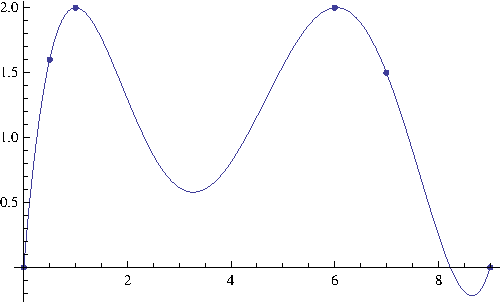
\includegraphics{plot.pdf}
\end{center}

\subsection*{Exercise 8.3}
Code:
\begin{lstlisting}
def midpoint(xlist,f):
    sum = 0
    for i in range(1,len(xlist)):
        sum += f((xlist[i-1]+xlist[i])/2)
    sum *= 2/float(n)
    return sum

def trapezoid(xlist,f):
    sum = 0
    for i in range(1,len(xlist)):
        sum += f(xlist[i-1]) + f(xlist[i])
    sum *= 1/float(n)
    return sum

def simpson(xlist,f):
    sum = 0
    for i in range(1,len(xlist)):
        sum += f(xlist[i-1]) + 4*f((xlist[i-1]+xlist[i])/2) + f(xlist[i])
    sum *= 1/(3.*float(n))
    return sum

def fa(x):
    y = cos(x)
    return y
def fb(x):
    y = 1/(1+100*x*x)
    return y

sola = 2*sin(1)
solb = 0.2*atan(10) 
nlist = [n for n in range(1,11)]
for n in nlist:
    xlist = [-1 + 2*x/float(n) for x in range(0,n+1)] #points (= #intervals+1)
    (ma,mb) = (midpoint(xlist,fa),midpoint(xlist,fb))
    (ma_error,mb_error) = (abs(ma-sola),abs(mb-solb))
    (ta,tb) = (trapezoid(xlist,fa),trapezoid(xlist,fb))
    (ta_error,tb_error) = (abs(ta-sola),abs(tb-solb))
    (sa,sb) = (simpson(xlist,fa),simpson(xlist,fb))
    (sa_error,sb_error) = (abs(sa-sola),abs(sb-solb))
    print "n = ",n," M(f) = ",ma," T(f) = ",ta," S(f) = ",sa
    print "error M(f) = ",ma_error," error T(f) = ",ta_error," error S(f) =",sa_error
\end{lstlisting}

\noindent In this exercise we use 3 different quadrature rules, midpoint, trapezoid and simpson to solve the integrals $\int_{-1}^{1} cos(x) dx$ and $\int_{-1}^{1} \frac{1}{1+100x^2} dx$ whose solutions are $2sin(1)$ and 
$0.2tan^{-1}(10)$ respectively. We subdivide the interval [-1,1] in n different steps. For each $n$ we calculate the error between the exact solution and the approximation. The results are given below for both integrals for $n$ from 2 up to 40 (and for $n = 10000$ to see the behavior for large $n$):

\begin{lstlisting}
For cos(x):
n =  2  error M(f) =  0.072223154165  error T(f) =  0.142639663748  error S(f) = 0.000602214860751
n =  4  error M(f) =  0.0176593209687  error T(f) =  0.0352082547914  error S(f) = 3.67957153313e-05
n =  6  error M(f) =  0.00781672207511  error T(f) =  0.0156117295986  error S(f) = 7.23818386561e-06
n =  8  error M(f) =  0.0043906637893  error T(f) =  0.00877446691134  error S(f) = 2.28688908743e-06
n =  10  error M(f) =  0.00280817912387  error T(f) =  0.00561355000178  error S(f) = 9.36081987479e-07
n =  12  error M(f) =  0.00194942877706  error T(f) =  0.00389750376176  error S(f) = 4.51264120738e-07
n =  14  error M(f) =  0.00143192539114  error T(f) =  0.00286312019923  error S(f) = 2.43527684018e-07
n =  16  error M(f) =  0.0010961648772  error T(f) =  0.00219190156102  error S(f) = 1.42731128916e-07
n =  18  error M(f) =  0.000866022718373  error T(f) =  0.00173177814382  error S(f) = 8.90976423751e-08
n =  20  error M(f) =  0.000701430398798  error T(f) =  0.00140268543895  error S(f) = 5.84528807579e-08
.
.
.
n =  10000  error M(f) =  2.80491230242e-09  error T(f) =  5.60981061604e-09  error S(f) = 0.0

For 1/(1+100x*x):
n =  2  error M(f) =  0.217302457938  error T(f) =  0.715675455238  error S(f) = 0.0936901797876
n =  4  error M(f) =  0.13882725147  error T(f) =  0.24918649865  error S(f) = 0.00948933476303
n =  6  error M(f) =  0.082650198587  error T(f) =  0.112123926716  error S(f) = 0.0177254901528
n =  8  error M(f) =  0.0469816494923  error T(f) =  0.0551796235903  error S(f) = 0.0129278917981
n =  10  error M(f) =  0.0259628706956  error T(f) =  0.0282487318884  error S(f) = 0.00789233650096
n =  12  error M(f) =  0.0141139395126  error T(f) =  0.0147368640643  error S(f) = 0.00449700498697
n =  14  error M(f) =  0.00760074310009  error T(f) =  0.00775754996168  error S(f) = 0.0024813120795
n =  16  error M(f) =  0.00407039292867  error T(f) =  0.00409898704902  error S(f) = 0.00134726626944
n =  18  error M(f) =  0.00217163206651  error T(f) =  0.00216687128221  error S(f) = 0.000725464283601
n =  20  error M(f) =  0.00115487861036  error T(f) =  0.00114293059639  error S(f) = 0.000388942208114
.
.
.
n =  10000  error M(f) =  6.5354166523e-11  error T(f) =  1.30707333845e-10  error S(f) = 0.0
\end{lstlisting}

\noindent The results above show that for the first integral the Simpson method converges much faster than the trapezoid or the midpoint methods. The trapezoid and midpoint methods give more or less similar results in terms of the error. For the evaluation of the second integral however all three methods converge nearly at the same rate for small $n$, with the simpson method being only slightly faster than the other two methods, however for large $n$ ($n>100$ the difference in the error increases, with $S(f)$ having smaller error than both the other methods, which have nearly the same error.\\
\noindent By increasing $n$ we can try to find $n$ such that the error is zero (within machine precision). For the first integral this happens for $S(f)$ at $n \approx 1406$. The other two methods do not reach zero error within $n = 10^5$. For the second integral $S(f)$ reaches zero at $n \approx 8800$, the other two methods again do not reach zero error within $n = 10^5$.
In conclusion both the approximations of the integrals converge much faster with the Simpson quadrature than with the other two quadrature methods, which have more or less an equal error. The approximation with the Simpson method converges faster for the first than for the second integral whereas the other two approximation converge slightly faster for the second integral than for the first integral.


\end{document}